\documentclass[12pt,fleqn]{book}

\usepackage{titlesec}
\usepackage{caption}

\titleformat{\chapter}[display]
  {\normalfont\huge\bfseries}{}{0pt}{\Huge}
\titlespacing{\chapter}
  {0pt}{10pt}{40pt}

	\newenvironment{amatrix}[1]{%
	  \left[\begin{array}{@{}*{#1}{r}|r@{}}
	}{%
	  \end{array}\right]
	}


\usepackage{amsmath,amssymb,amsfonts,graphicx,tasks,tikz,pgfplots}
\usetikzlibrary{arrows}
\pgfplotsset{compat=1.17}

\usepackage{tasks}
\settasks{
  label-width = 18pt
}
 
\makeatletter
 \def\@textbottom{\vskip \z@ \@plus 1pt}
 \let\@texttop\relax
\makeatother

\usepackage[letterpaper,margin=0.5in,footskip=.5cm]{geometry}

\setlength\parindent{0pt}

\usepackage{amsmath,amssymb,amsfonts,graphicx,tasks,tikz,pgfplots}
\usepackage{amsthm,thmtools}
\usetikzlibrary{arrows,quotes}

\usepackage{array}
\newcommand{\PreserveBackslash}[1]{\let\temp=\\#1\let\\=\temp}
\newcolumntype{C}[1]{>{\PreserveBackslash\centering}p{#1}}
\newcolumntype{R}[1]{>{\PreserveBackslash\raggedleft}p{#1}}
\newcolumntype{L}[1]{>{\PreserveBackslash\raggedright}p{#1}}

% Two-branch graph with equal scale and only max tick labels
% #1 = y1(x), #2 = y2(x), #3 = xmin, #4 = xmax, #5 = ymin, #6 = ymax,
% #7 = tick distance (ignored for equal scale), #8 = extra axis opts, #9 = plot opts
\newcommand{\graphpair}[9]{%
\begin{tikzpicture}[baseline=(current bounding box.north)]
  \begin{axis}[
    axis lines=middle,
    axis line style={very thick},
    grid style={thin,densely dotted,black!50},
    grid=major,
    xmin=#3-.2, xmax=#4+.2,
    ymin=#5-.2, ymax=#6+.2,
    xlabel=$x$, ylabel=$y$,
    axis equal image,
    % Only show largest tick values on each axis
    xticklabels={},
	yticklabels={},
	xtick distance=1, ytick distance=1,
	extra x ticks={#4},
	extra y ticks={#6},
    enlargelimits=false,
    % Allow optional extra axis settings
    #8
  ]
    \addplot[domain=#3:#4, samples=500, #9] (x,{#1});
    \addplot[domain=#3:#4, samples=500, #9] (x,{#2});
  \end{axis}
\end{tikzpicture}%
}


\newcommand{\graph}[8]{
\begin{tikzpicture}[baseline=(current bounding box.north)]
  \begin{axis}[
    axis lines=middle,
    axis line style={very thick},
    grid style={thin,densely dotted,black!50},
    grid=major,
      xtick distance=#6, ytick distance=#6,
      xmin=#2-.2, xmax=#3+.2,
      ymin=#4-.2, ymax=#5+.2,
      xlabel=$x$,
      ylabel=$y$,
    xticklabels={},
	yticklabels={},
	xtick distance=1, ytick distance=1,
	extra x ticks={#3},
	extra y ticks={#5},
      #7]
      \addplot[
      domain=#2:#3,
      samples=500,#8]
      (x,{#1});
    \end{axis}
  \end{tikzpicture}
}

\newcommand{\graphtwo}[9]{
\begin{tikzpicture}[baseline=(current bounding box.north)]
  \begin{axis}[
    axis lines=middle,
    axis line style={very thick},
    grid style={thin,densely dotted,black!50},
    grid=major,
      xtick distance=#7, ytick distance=#7,
\usepackage{amsmath,amssymb,amsfonts,amsthm,thmtools}
      xmin=#3-.2, xmax=#4+.2,
      ymin=#5-.2, ymax=#6+.2,
      xlabel=$x$,
      ylabel=$y$,
      #8]
      \addplot[
      domain=#3:#4,
      samples=500,#9]
      (x,{#1});
      \addplot[
      domain=#3:#4,
      samples=500,#9]
      (x,{#2});
    \end{axis}
  \end{tikzpicture}
}

\newcommand{\curve}[7]{% function, xmin, xmax, ymin, ymax, 
\begin{tikzpicture}[baseline=(current bounding box.north)]
  \begin{axis}[
    axis lines=middle,
    axis line style={very thick},
    grid style={thin,densely dotted,black!50},
    grid=major,
    xticklabels={},
	yticklabels={},
	xtick distance=1, ytick distance=1,
	extra x ticks={#3},
	extra y ticks={#5},
      xmin=#2-.2, xmax=#3+.2,
      ymin=#4-.2, ymax=#5+.2,
      xlabel=$x$,
      ylabel=$y$,
      #6]
      \addplot[
      domain=#2:#3,
      samples=500,#7]
      (x,{#1});
    \end{axis}
  \end{tikzpicture}
}

\newcommand{\blankgraph}[6]{
\begin{tikzpicture}[baseline=(current bounding box.north)]
  \begin{axis}[
    width=#5in,height=#6in,
    axis lines=middle,
    axis line style={very thick},
    grid style={thin,densely dotted,black!50},
    grid=major,
    xticklabels={},
	yticklabels={},
	xtick distance=1, ytick distance=1,
	extra x ticks={#2},
	extra y ticks={#4},
      xtick distance=1, ytick distance=1,
      xticklabels={1},
      yticklabels={1},
      xmin=#1-.2, xmax=#2+.2,
      ymin=#3-.2, ymax=#4+.2,
      xlabel=$x$,
      ylabel=$y$]
    \end{axis}
  \end{tikzpicture}
}

\newcommand{\blankaxes}[2]{
\begin{tikzpicture}[baseline=(current bounding box.north)]
  \begin{axis}[
    width=#1in,height=#2in,
    axis lines=middle,
    axis line style={very thick},
    grid=major,
    xtick distance=2, ytick distance=2,
    xmin=-1, xmax=1,
    ymin=-1, ymax=1,
    xlabel=$x$,
    ylabel=$y$]
  \end{axis}
\end{tikzpicture}
}

\newcommand{\ds}{\displaystyle}

\newcommand{\lr}[1]{\left(#1\right)}

% \usepackage{amsthm}
% \theoremstyle{definition}
% \newtheorem{problem}{}
% \counterwithin*{problem}{section}
% \renewcommand{\theproblem}{\thesubsection.\arabic{problem}}
%
% \newtheorem*{solutionx}{\thesolutionnumber}
% \ExplSyntaxOn
% \tl_new:N \g_gargantuar_solution_tl
%
% \NewDocumentEnvironment{solution}{+b}
%  {
%   \tl_gput_right:Nx \g_gargantuar_solution_tl
%    {
%     \printsolution{\theproblem}{ \exp_not:n { #1 } }
%    }
%  }
%  {}
% \NewDocumentCommand{\printsolutions}{}
%  {
%   \tl_use:N \g_gargantuar_solution_tl
%   \tl_gclear:N \g_gargantuar_solution_tl
%  }
% \NewDocumentCommand{\printsolution}{m +m}
%  {
%   \cs_set:Npn \thesolutionnumber { #1 }
%   \begin{solutionx} #2 \end{solutionx}
%  }
% \ExplSyntaxOff
% \makeatother
%
% \newcommand{\prb}[1]{\begin{problem}#1\end{problem}}
% \newcommand{\sol}[1]{\begin{solution}#1\end{solution}}
% =============================
% TCOLORBOX CONFIGURATION
% =============================

\usepackage{tcolorbox}

\definecolor{black}{rgb}{0,0,0}
\definecolor{dark-gray}{rgb}{.15,.15,.15}
\definecolor{light-gray}{rgb}{.85,.85,.85}
\definecolor{white}{rgb}{1,1,1}

\makeatletter
\newcommand*\ifcounter[1]{%
	\ifcsname c@#1\endcsname
		\expandafter\@firstoftwo
	\else
		\expandafter\@secondoftwo
	\fi
}
\makeatother

\tcbuselibrary{theorems}

\ifcounter{unit}{
	\newtcbtheorem{defn}{Definition \theunit.\hspace{-.3em}}{
		colback=light-gray,colframe=dark-gray,coltitle=white,coltext=black,fonttitle=\bfseries,before skip=20pt plus 2pt,after skip=20pt plus 2pt}{th}
}{
	\newtcbtheorem{defn}{Definition}{
		colback=light-gray,colframe=dark-gray,coltitle=white,coltext=black,fonttitle=\bfseries,before skip=20pt plus 2pt,after skip=20pt plus 2pt}{th}
}

\ifcounter{unit}{
	\newtcbtheorem{thm}{Theorem \theunit.\hspace{-.3em}}{
		colback=light-gray,colframe=dark-gray,coltitle=white,coltext=black,fonttitle=\bfseries,before skip=20pt plus 2pt,after skip=20pt plus 2pt}{th}
}{
	\newtcbtheorem{thm}{Theorem}{
		colback=light-gray,colframe=dark-gray,coltitle=white,coltext=black,fonttitle=\bfseries,before skip=20pt plus 2pt,after skip=20pt plus 2pt}{th}
}



\pagestyle{plain}
\usepackage[lastexercise,answerdelayed]{exercise}
\usepackage{totcount}
\regtotcounter{Exercise} % register the counter for getting the total
\usepackage{chngcntr}
\counterwithin{Exercise}{chapter}
\counterwithin{Answer}{chapter}
\usepackage{xassoccnt}
\NewTotalDocumentCounter{totalex}
\usepackage{titleref}
\usepackage{etoolbox}

%EXERCISE START

\renewcommand{\ExerciseHeader}{ \stepcounter{totalex}\ifnumcomp{\value{Exercise}}{=}{1}{\ifnumcomp{\thechapter}{=}{1}{}{\vspace{10pt}}\noindent\Large\textbf{Exercises}\par\vspace{10pt}}{}\noindent\normalsize\bfseries\ExerciseHeaderNB\ExerciseHeaderDifficulty.}
\renewcommand{\AnswerHeader}{\ifnumcomp{\value{Exercise}}{=}{1}{\ifnumcomp{\thechapter}{=}{1}{}{\vspace{10pt}}\noindent\Large\textbf{Section\ \thechapter\ Solutions}\par\vspace{10pt}}{}\noindent\normalsize\bfseries\ExerciseHeaderNB.\ }

\usepackage{hyperref}

\newcommand{\prb}[1]{\begin{Exercise}#1\end{Exercise}}
\newcommand{\sol}[1]{\begin{Answer}#1\end{Answer}}

\begin{document}
\noindent
\thispagestyle{empty}
Grade 10 Advanced Math \hfill Name: \hspace{2in}
\medskip\hrule
\noindent

\vfill

\begin{center}
    {\bf \huge Chapter 3: Radicals and Exponents}
\end{center}

\vfill
\vfill

\clearpage

\setcounter{page}{1}

{\bf \huge Introduction }
\\[1in]
In the first chapter, we dealt with functions that could be sketched as a straight line.  We observed how they intersected with each other, and how we can use algebra to describe those intersections.
\\[1em]
In the second chapter, we learned about polynomial functions, namely quadratics, and how they can be graphed.  We spent a great deal of time finding roots of a quadratic, and even learned about imaginary numbers.
\\[1em]
In this chapter, we will learn about the inverse of a quadratic -- a radical.  We will learn how to play with these kinds of numbers, what \emph{kinds} of numbers they can be, and how to express them in various ways.
\\[1em]
Try this warm up to see if you can get all of these facts right.
\begin{tasks}(2)
    \task $3^2=$
    \task $(-3)^2=$
    \\[1in]
    \task If $x^2=9,$ then $x=$
    \task $\sqrt 9 =$
    \\[1in]
    \task $\sqrt{x^2}=$
    \task $(\sqrt x)^2=$
\end{tasks}
\clearpage
\chapter{1. Relations, Functions, One-to-one}
We have seen several types of function in this class so far.  The first type, and most straightforward was the linear function.  Then we realized that if we multiplied two linear functions together, we got a quadratic function.  There are also higher-degree polynomial functoins that we briefly explored in the last chapter.
\\[1em]
It turns out that functions are the life-blood of a lot of mathematics.  Most of mathematics can be described using the language of functions.
\\[1em]
But not all equations can be described as a function.  It is probably a  good idea to remind ourselves what exactly a function is!
\begin{defn}{Function}{}
    A function is a rule that takes as input one value and outputs another value, related to the input.  If $x$ is the input of function $f$, and $y$ is the output of the function, then we write
    \[
        y=f(x)
    \]
\end{defn}
It is critical to understand that for every single input, there is a single output.  A function fails to be a function if you were to input a single value and get back \emph{two} or more values.
\\[1em]
Consider the following functions.
\begin{tasks}(4)
    \task
    $f(x)=x^2$
    \task
    $f(x)=(x-2)(x+1)^2$
    \task
    $y=x-4$
    \task
    $g(x)=\sqrt x$
\end{tasks}
Use Desmos to help you graph the above functions below.
\\[1em]
\blankgraph{-4}{4}{-4}{4}{2.3}{2.3}
\blankgraph{-4}{4}{-4}{4}{2.3}{2.3}
\blankgraph{-4}{4}{-4}{4}{2.3}{2.3}
\blankgraph{-4}{4}{-4}{4}{2.3}{2.3}
\\[1em]
Some equations in math, however, are not best described as a function.  Sometimes if I give you one input, you may want two outputs.
\\[1em]
The following are not functions:
\begin{tasks}(2)
    \task
    $y^2=x$
    \task
    $x^2+y^2=1$
    \task
    $x^3+y^2=xy$
    \task
    $y=\pm x$
\end{tasks}
Use Desmos to help you graph these functions.  Try to see if you can visualize \emph{exactly} what makes these equations non-functions.
\\[1em]
\blankgraph{-4}{4}{-4}{4}{2.3}{2.3}
\blankgraph{-4}{4}{-4}{4}{2.3}{2.3}
\blankgraph{-4}{4}{-4}{4}{2.3}{2.3}
\blankgraph{-4}{4}{-4}{4}{2.3}{2.3}
\\[1em]
\begin{defn}{Relation}{}
    An equation that has two or more variables is called a relation.  Most relations are between two variables, $x$ and $y$.  If the relation $R$ has a solution $x=a$ and $y=b$, then the the relation can be graphed by plotting $(a,b)$, and all other solutions to the equation.  Furthermore, we can write $a R b$ and say $a$ is related to $b$.
\end{defn}
So all of the above equations are relations because they represent a relationship between $x$ and $y$.  When Desmos graphs these, they are finding all possible solutions to the equation, and plotting each point, one by one.
\\[1em]
We can also describe a relation by means of a mapping diagram.
\\[1em]
\mappingdiagram{1,2,3}{a,b,c}{1/1,2/2,3/3}
\\[1em]
The above mapping diagram indicates that we have two sets, $\{a, b, c\}$, and $\{1, 2, 3\}$.
The first set is referred to as our domain, and the second set is called the range.
\begin{defn}{Domain and Range}{}
    The domain of a relation is the collection of objects that go \emph{into} the relation, and the range is the collection of objects that come \emph{out of} the relation.
\end{defn}
The mapping diagram indicates that $a$ is related to $1$, (or $a$ is 'mapped' to $1$), $b$ is related to $2$, and $c$ is related to $3$.  We could also write $aR1$, $bR2$, and $cR3$.  We can also say that the following ordered pairs describe the relation: $(a,1), (b,2),$ and $(c,3)$.
\\[1em]
Describe the following relation in all of the ways you know how:
\\[1em]
\mappingdiagram{1,2,3}{a,b,c}{1/2,2/3,3/1,2/1}
\\[1em]
Draw the mapping diagram of the relation described by the following ordered pairs:
\[
    (a,4),(b,3),(c,0),(a,3),(8,\alpha)
\]
There is a quick way of determining when a graph represents a function and when it doesn't.
\begin{defn}{Vertical Line Test}{}
    Given the graph of a relation, if there exists a vertical line that overlaps the curve of the graph more than once, then the relation is not a function.  If no such vertical line exists, then the relation is a function.
\end{defn}
Use the Vertical Line Test to determine which of these graphs represents a relation that is a function, and which is a relation that is \emph{not} a function.
\begin{tasks}(2)
    \task \graph{0.2*(x + 2)*(x - 1)*(x - 3)}{-4}{6}{-6}{6}{1}{}{}
    \task \graphpair{1 + 3*sqrt(1 - (x/2)^2)}{1 - 3*sqrt(1 - (x/2)^2)}{-2}{2}{-2.5}{4.5}{0.5}{}{}
    \task \graphpair{2}{-(2 - (x - 1)^2)}{-3}{5}{-4}{4}{1}{}{}
    \task \graph{(x - 1)^2 - 2}{-4}{6}{-4}{6}{1}{}{}
    \task \graph{abs(x)}{-5}{5}{-1}{5}{1}{}{}
    \task \graphpair{sqrt(9-x^2)}{-sqrt(9-x^2)}{-3}{3}{-3}{3}{1}{}{}
    \task \graph{-0.5*x + 2}{-6}{6}{-4}{6}{1}{}{}
    \task \graphpair{1 + sqrt(x + 2)}{1 - sqrt(x + 2)}{-2}{7}{-3}{5}{1}{}{}
\end{tasks}

As you may be able to sense, a function is a special type of relation.  But is there something even more special?  Are there types of functions are even more exclusive?  It turns out: yes.  These functions are called one-to-one functions.

Recall that the feature that a relation requires is that for every one input there is exactly one output. For a function to be one to one, we require the following.
\begin{defn}{One-to-one Function}{}
    A function is said to be one-to-one if for every single \emph{output}, there is exactly one \emph{input}.  Symbolically, we can say:
    \[
        f(a)=f(b) \text{ implies } a=b.
    \]
    In other words, the only way that two outputs can be the same ($f(a)$ and $f(b)$), is if they are not two outputs at all -- that they are indeed from the same input ($a$ and $b$).
\end{defn}

It is useful to remember that one-to-one functions are \emph{all} functions, and all functions are relations.  But not all relations are function, and not all functions are one-to-one.
\\[1em]
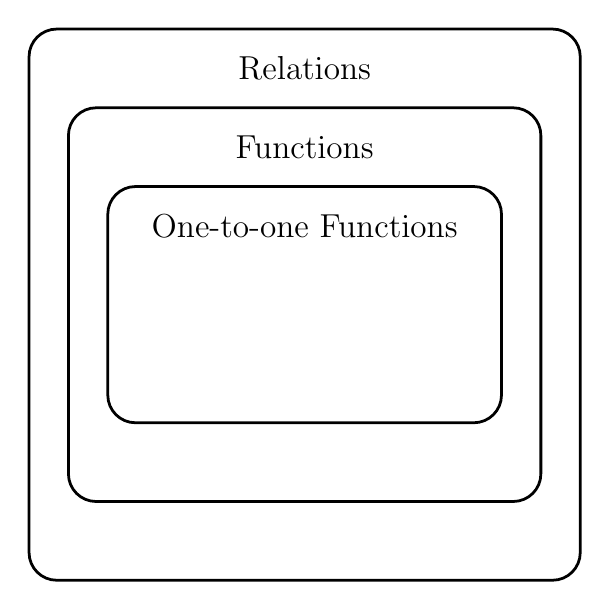
\begin{tikzpicture}[font=\large, line width=1pt]

    % Outer rectangle: Relations
    \node[draw, rounded corners=10pt, minimum width=7cm, minimum height=7cm, anchor=center] (relations) at (0,0) {};

    % Middle rectangle: Functions
    \node[draw, rounded corners=10pt, minimum width=6cm, minimum height=5cm, anchor=center] (functions) at (0,0) {};

    % Inner rectangle: One-to-one Functions
    \node[draw, rounded corners=10pt, minimum width=5cm, minimum height=3cm, anchor=center] (one2one) at (0,0) {};

    % Labels (placed near the top of each rectangle)
    \node at (0,3) {Relations};
    \node at (0,2) {Functions};
    \node at (0,1) {One-to-one Functions};

\end{tikzpicture}

\begin{defn}{Horizontal Line Test}{}
    Given the graph of a function, if there exists a horizontal line that overlaps the curve of the graph more than once, then the function is not one-to-one.  If no such horizontal line exists, then the function is one-to-one.
\end{defn}
Explain why the horizontal line test works.
\clearpage
Use the horizontal line test to determine which of the following functions are one-to-one.
\begin{tasks}(2)
    \task \graph{0.2*(x + 2)*(x - 1)*(x - 3)}{-4}{6}{-6}{6}{1}{}{}
    \task \graph{(x - 1)^2 - 2}{-4}{6}{-4}{6}{1}{}{}
    \task \graph{abs(x)}{-5}{5}{-1}{5}{1}{}{}
    \task \graph{-0.5*x + 2}{-6}{6}{-4}{6}{1}{}{}
    \task \graph{-0.1*x^3 + 2}{-6}{6}{-4}{6}{1}{}{}
    \task \graph{5*sin(.8*deg(x))}{-6}{6}{-6}{6}{1}{}{}
\end{tasks}
\clearpage
\prb{
    In your own words, explain the following terms.
    \begin{tasks}(5)
        \task domain
        \task range
        \task relation
        \task function
        \task one-to-one
    \end{tasks}
    You may want to include definitions for these items as well as for range and function.
    \\[3in]
}
\prb{
    What is the rule that you use to determine whether a relation (mapped or in a table) represents a function?
    \\[1in]
}
\prb{
    In your own words, explain what the vertical line test is used for and how it works.
    \\[1in]
}
\prb{
    Determine whether the following relations are functions. Justify your answer.
    \begin{tasks}(2)
        \task $\mathrm{A}=\{(1,2),(1,7),(1,8),(1,9),(1,10)\}$
        \task $y=-x+3$
    \end{tasks}
    \clearpage
}
\prb{
    The physical education teacher calls out the first name of 6 students in a class (Aiden, Brady, Chad, Chad, Devon, Everett) and numbers them 1 through 6.
    If this information were written as ordered pairs (number, name), would this represent a function or a non-function? Explain.
    \\[1in]
}
\prb{State the domain and range of the following relation.
    \[
        A=\{(1,2)(3,4)(5,6)(7,8)\}
    \]
    \vspace{1in}
}
\sol{The domain is all possible $x$-values.
    \[
        \begin{aligned}
             & D=\{1,3,5,7\} \\
             & R=\{2,4,6,8\}
        \end{aligned}
    \]
}
\prb{
    The provincial sales tax in Manitoba is $7 \%$ of the list price. Write a relation to illustrate the relationship between the list price and the cost of the item to the consumer. State the domain and range of this relation.
    \\[2in]
}
\sol{
    Some ordered pairs for this relation are $(\$ 10.00, \$ 10.70),(\$ 20.00, \$ 21.40)$, ( $\$ 0.70, \$ 0.75$ ). The possible list price and cost pairs are endless. To simplify, you could specify the relationship using a formula with variables to represent the relationship. The cost is the list price plus 7\% of the list price.
        \[
            C=L+0.07 L
        \]
        or
        \[
            C=1.07 L
        \]
        Where $C$ is the cost to the consumer (price after $\operatorname{tax})$ and $L$ is the list price.
        The domain of this relation is the set of all possible list prices, and the range is the resulting cost to the consumer when tax is added to the list price. These values will be a subset of positive real numbers.
        \\[1em]
        From the above example it is obvious that the domain (the list price of an item) affects the range (the total cost). You can think of it in terms of input and output. The $x$-value that is put into the relation determines the $y$-value that comes out. Organized as a table of values, it may look like this:
    \[
        \begin{array}{|c|c|}
            \hline \text { Input } & \text { Output } \\
            \hline L               & C                \\
            \hline \$ 10.00        & \$ 10.70         \\
            \hline \$ 20.00        & \$ 21.40         \\
            \hline \$ 0.70         & \$ 0.75          \\
            \hline
        \end{array}
    \]
}
\prb{
    Given the following ordered pairs, state the domain and range of the relation.
    \[
        \{(1,4)(2,6)(3,8)(4,10)\}
    \]
    \clearpage}
\sol{Domain: $\{ 1,2,3,4 \}$, range: $\{ 4,6,8,10 \}$.}
\prb{
    Determine if the following ordered pairs represent functions or relations.
    \begin{tasks}(2)
        \task $\{(0,1),(1,2),(2,3),(3,4),(4,5)\}$
        \\[1in]
        \task $\{(2,-3),(2,5),(2,0),(2,1),(2,-2)\}$
        \\[1in]
        \task $\{(-4,-1),(3,-1),(0,-1),(-1,-1),(5,-1)\}$
        \\[1in]
        \task $\{(5,3),(4,3),(-3,3),(0,5),(-3,-1)\}$
        \\[1in]
        \task $\{(-2,4),(-1,1),(0,0),(1,1),(2,4)\}$
        \\[1in]
    \end{tasks}
}
\sol{
    \begin{tasks}(2)
        \task This is a function and a relation because each $x$-value has only one possible $y$-value.
        \task This is only a relation because the input of 2 has a variety of possible outputs.
        \task This is a function and a relation because each element in the domain has only one possible value for its range.
        \task This relation is a non-function. The input of -3 has two possible outputs: 3 and -1 .
        \task This represents a relation and a function. The value of 1 is the output in two ordered pairs $(-1,1)$ and $(1,1)$, but each input has only one possible output so it still fits the definition of a function.
    \end{tasks}
}

\prb{Decide whether the relations shown are one-to-one. Justify.
    \begin{tasks}(2)
        \task
        \mappingdiagram{1,2,3}{a,b,c}{1/1,2/2,3/3}
        \task
        \mappingdiagram{1,2,3,4}{p,q,r}{1/1,2/1,3/2,4/3}
    \end{tasks}
}
\sol{
    \begin{tasks}(2)
        \task Each output is hit by exactly one input, and no output repeats. \textbf{Yes}, it is one-to-one.
        \task
        Outputs repeat: $p$ is the image of both 1 and 2, so different inputs share an output. \textbf{Not} one-to-one.
    \end{tasks}
}
\prb{The diagram below is not one-to-one. What is the \emph{fewest} number of domain elements you must remove to make it one-to-one? Give one possible choice.
    \mappingdiagram{A,B,C,D}{1,2,3}{1/1,2/2,3/2,4/3}
}
\sol{Output \(2\) has two preimages (B and C). Remove \emph{one} of \(\{B,C\}\). After removing one, each output has at most one preimage, so it becomes one-to-one.}

\prb{Let \(f(x)=2x+3\). Is \(f\) one-to-one on \(\mathbb{R}\)? Show work.
    \\[1in]
}
\sol{\(f(x_1)=f(x_2)\Rightarrow 2x_1+3=2x_2+3\Rightarrow x_1=x_2\). Therefore \(f\) is \textbf{one-to-one} (its graph also passes the horizontal line test).}

\prb{Consider \(g(x)=x^2-4\) on the domain \(\mathbb{R}\). Is \(g\) one-to-one? If not, give a domain restriction that makes it one-to-one and state the.
    \\[1in]
}

\sol{\(g\) is \textbf{not} one-to-one since \(g(2)=g(-2)=0\). Restrict to \(x\ge 0\) (or \(x\le 0\)) to make it one-to-one.}

\prb{Is \(h(x)=|x-2|\) one-to-one on \(\mathbb{R}\)? If not, give a largest interval on which it is one-to-one.
    \\[1in]
}
\sol{Not one-to-one (\(h(1)=h(3)=1\)). On \([2,\infty)\) it is one-to-one.}

        \prb{The function \(p(x)=\dfrac{3x-5}{2}\). Explain why \(p\) is one-to-one}
        \sol{Linear with nonzero slope \(\tfrac{3}{2}\Rightarrow\) strictly increasing \(\Rightarrow\) one-to-one.}

        \prb{For which values of \(a\) is \(f(x)=ax+b\) one-to-one on \(\mathbb{R}\)? Justify.
            \\[1in]
        }
        \sol{If \(a=0\), \(f(x)=b\) is constant (not one-to-one). If \(a\ne0\), it’s strictly monotonic, so \textbf{one-to-one}. Thus: \(a\ne0\).}

        \prb{Determine whether the piecewise function
            \[
                f(x)=\begin{cases}
                    x+1, & x<0,  \\
                    1-x, & x\ge0
                \end{cases}
            \]
            is one-to-one on \(\mathbb{R}\).
            \\[1in]
        }
        \sol{No. For example, \(f(-1)=0\) and \(f(1)=0\), so two different inputs give the same output. \(\Rightarrow\) not one-to-one.}

        \prb{A table of values is given:
            \[
                \begin{array}{c|ccccc}
                    x    & -2 & -1 & 0 & 1 & 2 \\\hline
                    f(x) & 3  & 5  & 3 & 7 & 9
                \end{array}
            \]
            Is \(f\) one-to-one? If not, remove the \emph{fewest} entries to make it one-to-one and rewrite the table.
            \\[1in]}
        \sol{Not one-to-one since \(f(-2)=f(0)=3\). Remove either \((-2,3)\) or \((0,3)\). One possible one-to-one table:
            \(\{(-1,5),(0,3),(1,7),(2,9)\}\).}



        \chapter{2. Inverse Functions}
        A common theme in mathematics is learning how to do something backwards.  When you first learned how to add, it wasn't long before you learned how to undo adding: you learned how to subtract.  After you learned how to multiply, you learned how to divide.  When you solve an equation, you repeatedly undo the operations done to your variable.  When you learn about the derivative in calculus, you will also learn about the antiderivative, which undoes the derivative operation.
        \\[1em]
It may be of interest to us to find a way to undo a function.  This is called the inverse.
\begin{defn}{Inverse Function}{}
    The inverse of a function $f(x)$, if it exists, is the unique function $f^{-1}(x)$ such that
    \[
        f(f^{-1}(x))=f^{-1}(f(x))=x.
    \]
    In other words, the inverse of $f$ undoes what $f$ does to $x$
\end{defn}
For example, the inverse of $f(x)=\frac12 x - 2$ is $f^{-1}(x)=2x+4$.  Why is that?
\subsection*{How to find the inverse of a function}
To find the inverse of a function, provided it exists (more on that later), we take the following steps:
\begin{enumerate}
    \item write the function as $y$ in terms of $x$
    \item replace $x$ and $y$
    \item solve for $y$
    \item profit.
\end{enumerate}
Find the inverse of $f(x)=3x-12$ and verify that it is indeed the inverse.
\\[2in]
\subsection*{Which functions have inverses?}
Not all functions have inverses.  Take $f(x)=x^2$ for example.  Since $f(2)=4$ and $f(-2)=4$, if our inverse $f^{-1}$ \emph{did} exist, what could $f^{-1}(4)$ be equal to?  It would have to undo both of the mappings that map to 4.
\begin{thm}{Only one-to-one functions have inverses}{}
    If a function $f(x)$ is one-to-one, then $f^{-1}(x)$ exists.  When this happens, the domain and range of $f$ are the range and domain of $f^{-1}$, respectively.  In other words, the domain and range swap.
\end{thm}
Why do you think we need $f$ to be one-to-one in order to find its inverse?
\\[2in]
Find the inverse of the following functions:
\begin{tasks}(3)
    \task $f(x) = 2x + 3 $\\[2in]
    \task $g(x) = -x + 1 $\\[2in]
    \task $h(x) = \tfrac{1}{2}x - 4 $\\[2in]
    \task $p(x) = -3x - 2 $\\[2in]
    \task $q(x) = 4x $\\[2in]
    \task $r(x) = -\tfrac{2}{3}x + 5$\\[2in]
\end{tasks}

\prb{
    Algebraically determine the equation of the inverse of each function.
    \begin{tasks}(2)
        \task $f(x)=7 x$
        \\[2.5in]
        \task $f(x)=-3 x+4$
        \\[2in]
        \task $f(x)=\frac{x+4}{3}$
        \\[2.5in]
        \task $f(x)=\frac{x}{3}-5$
        \\[2in]
        \task $f(x)=5-2 x$
        \\[2.5in]
        \task $f(x)=\frac{1}{2}(x+6)$
        \\[2in]
    \end{tasks}
}
\sol{
    \begin{tasks}(2)
        \task
        \begin{align*}
            f(x)      & =7 x           \\
            y         & =7 x           \\
            x         & =7 y           \\
            y         & =\frac{1}{7} x \\
            f^{-1}(x) & =\frac{1}{7} x
        \end{align*}
        \task
        \begin{align*}
            f(x)      & =-3 x+4            \\
            y         & =-3 x+4            \\
            x         & =-3 y+4            \\
            x-4       & =-3 y              \\
            y         & =-\frac{1}{3}(x-4) \\
            f^{-1}(x) & =-\frac{1}{3}(x-4)
        \end{align*}
        \task
        \begin{align*}
            f(x)      & =\frac{x+4}{3} \\
            y         & =\frac{x+4}{3} \\
            x         & =\frac{y+4}{3} \\
            3 x       & =y+4           \\
            y         & =3 x-4         \\
            f^{-1}(x) & =3 x-4
        \end{align*}
        \task
        \begin{align*}
            f(x)      & =\frac{x}{3}-5 \\
            y         & =\frac{x}{3}-5 \\
            x         & =\frac{y}{3}-5 \\
            x+5       & =\frac{y}{3}   \\
            y         & =3(x+5)        \\
            f^{-1}(x) & =3(x+5)
        \end{align*}
        \task
        \begin{align*}
            f(x)      & =5-2 x             \\
            y         & =5-2 x             \\
            x         & =5-2 y             \\
            x-5       & =-2 y              \\
            y         & =-\frac{1}{2}(x-5) \\
            f^{-1}(x) & =-\frac{1}{2}(x-5)
        \end{align*}
        \task
        \begin{align*}
            f(x)      & =\frac{1}{2}(x+6) \\
            y         & =\frac{1}{2}(x+6) \\
            x         & =\frac{1}{2}(y+6) \\
            2 x       & =y+6              \\
            y         & =2 x-6            \\
            f^{-1}(x) & =2 x-6
        \end{align*}
    \end{tasks}
}
\clearpage
\prb{Assume that $f$ is a one-to-one function.
    \begin{tasks}(2)
        \task If $f(2)=7$, find $f^{-1}(7)$.
        \\[2in]
        \task If $f^{-1}(3)=-1$, find $f(-1)$.
        \\[2in]
        \task If $f(5)=18$, find $f^{-1}(18)$.
        \\[2in]
        \task If $f^{-1}(4)=2$, find $f(2)$.
        \\[2in]
        \task If $f(x)=5-2 x$, find $f^{-1}(3)$.
        \\[2in]
        \task If $g(x)=x^2+4 x$ with $x=-2$, find $g^{-1}(5)$.
        \\[2in]
    \end{tasks}

}
\clearpage
\prb{
    Find the inverse function of $f$.
    \begin{tasks}(2)
        \task $f(x)=3 x+5$
        \\[2in]
        \task $f(x)=7-5 x$
        \\[2in]
        \task $f(x)=5-4 x^3$
        \\[2in]
        \task $f(x)=3 x^3+8$
        \\[2in]
        \task $f(x)=\frac{1}{x+2}$
        \\[2in]
        \task $f(x)=\frac{x-2}{x+2}$
        \\[2in]
        \task $f(x)=\frac{x}{x+4}$
        \\[2in]
        \task $f(x)=\frac{3 x}{x-2}$
        \\[2in]
        \task $f(x)=\frac{2 x+5}{x-7}$
        \\[2in]
        \task $f(x)=\frac{4 x-2}{3 x+1}$
        \\[2in]
        \task $f(x)=\frac{2 x+3}{1-5 x}$
        \\[2in]
        \task $f(x)=\frac{3-4 x}{8 x-1}$
        \\[2in]
        \task $f(x)=4-x^2, \quad x \geq 0$
        \\[2in]
        \task $f(x)=x^2+x, \quad x \geq-\frac{1}{2}$
        \\[2in]
        \task $f(x)=x^6, \quad x \geq 0$
        \\[2in]
        \task $f(x)=\frac{1}{x^2}, x>0$
        \\[2in]
        \task $f(x)=\frac{2-x^3}{5}$
        \\[2in]
        \task $f(x)=\left(x^5-6\right)^7$
        \\[2in]
        \task $f(x)=\sqrt{5+8 x}$
        \\[2in]
        \task $f(x)=2+\sqrt{3+x}$
        \\[2in]
        \task $f(x)=2+\sqrt[3]{x}$
        \\[2in]
        \task $f(x)=\sqrt{4-x^2}, \quad 0 \leq x \leq 2$
        \\[2in]
    \end{tasks}
}
\chapter{3. The Radical Function}
The last section was a short detour to talk about the radical function.  In order to fully understand the radical function, we must be familiar with the following ideas:
\begin{itemize}
    \item domain
    \item range
    \item one-to-one
    \item inverse
\end{itemize}
Since the function $f(x)=x^2$ is not one-to-one, we cannot take its inverse.  But what would happen if we were to \emph{restrict} its domain to the positive real numbers only?
\\[1em]
Graph $y=x^2$ over the domain $x\ge 0$.
\[
    \blankgraph{-1}{10}{-1}{10}{3}{3}
\]
If we define this function, which is only defined for values $x\ge 0$ as $g(x)$, then we have the very convenient fact that $g$ is one-to-one.
\\[1em]
How do we know this?
\\[2in]
\begin{defn}{The radical function}{}
    Let $g(x)=x^2$ over the restricted domain $x\ge 0$, making $g$ one-to-one.  The function $g^{-1}(x)$ is called the \emph{square root} function and is in the family of radical functions.  We usually write:
    \[
        g^{-1}(x)=\sqrt{x}
    \]
\end{defn}
Wait$\ldots$ it's taken us three chapters to define $\sqrt x$?  Yes.
\\[1em]
Now let's revisit the blurb from the first page of this book:
\begin{tasks}(2)
    \task $3^2=$
    \task $(-3)^2=$
    \\[1em]
    \task If $x^2=9,$ then $x=$
    \task $\sqrt 9 =$
    \\[1em]
    \task $\sqrt{x^2}=$
    \task $(\sqrt x)^2=$
    \\[1em]
\end{tasks}
All of this is to say that if $y=\sqrt x$ then $y^2=x$, but just because $y^2=x$ does not mean that $y=\sqrt x$.
\\[1em]
Explain the above sentence in your own words, and give an example of $x$ and $y$ that satisfy that sentence.
\\[2in]
Graph the function $y=\sqrt x$
\[
    \blankgraph{-1}{10}{-1}{10}{3}{3}
\]
Use this graph to approximate $\sqrt 7$.
\chapter{4. Number Systems}
Use Desmos to help you graph $y=\sqrt x$ as perfectly as possible.  It may help to remember that the square root function is the inverse of $y=x^2$ over the restricted domain of $x\ge 0$, so its shape should be very similar.
\[
    \blankgraph{-1}{10}{-1}{10}{3}{3}
\]
When we graph the function $y=\sqrt x$ we see the following point on the graph:
\begin{itemize}
    \item $(0,0)$ since $0^2=0$
    \item $(1,1)$ since $1^2=1$
    \item $(4,2)$ since $2^2=4$
    \item $(9,3)$ since $3^2=9$
    \item and so on
\end{itemize}
But there are \emph{so many more} points on this function.  In fact, between any two different points on the graph, there are \emph{infinitely many} points in between them. What do some of those points look like?  Try seeing what happens to $y$ when $x=7$.

Are there any integers whose square root is not an integer?

\begin{defn}{Rational numbers}{}
    A rational number is a number that can be written as the ratio of two integers $a$ and $b$, provided that $b\ne 0$.  The set of all rational numbers is denoted $\mathbb Q$, because $Q$ stands for quotient.  In symbols,
    \[
        \mathbb Q = \left\{ \frac ab : a, b \in \mathbb Z \right\}
    \]
\end{defn}
It turns out that the square root of an integer can be a very strange kind of number.
\begin{thm}{The irrationality of $\sqrt 2$}{}
    The square root of 2 is not a rational number.
\end{thm}
Why is this?
\\[4in]
\clearpage
It turns out that there are all kinds of different numbers out there.
To recap, we have the following sets of numbers:
\begin{itemize}
    \item
          The Natural Numbers $\mathbb N = \{0, 1, 2, 3, 4, \ldots \}$.
          \\
          These are sometimes called the counting numbers.  Some definitions of the natural numbers do not include zero (but they're wrong!).  In this class we will use 0 as the least element.  Regardless of the definition, the Natural Numbers have a smallest element, but no greatest element.
    \item
          The Integers $\mathbb Z = \{ \ldots -3, -2, -1, 0, 1, 2, 3, \ldots \}$.
          \\
          The integers have no least element and no greatest element.  It includes positive numbers, negative numbers, and zero.  There are no decimal numbers (unless you include decimals that end in .0) in $\mathbb Z$.
    \item
          The Rational Numbers $\mathbb Q = \{\frac ab : a,b\in\mathbb Z, b\ne 0 \}$.
          \\
          A rational number is a value that can be expressed as the ratio of two integers, so long as we do not divide by 0.  These values can be represented by fractions or decimals.  When a rational number is in decimal form, it is either a repeating decimal or a terminating decimal.  Conversely, all terminating decimals and repeating decimals are rational.
    \item
          Irrational Numbers
          \\
          These are numbers that cannot be written as the ratio of two integers.  This set can be harder to describe because irrational numbers are defined by a property that they don't have.  Irrational numbers in decimal form do not terminate and do not repeat.  Examples include $\sqrt 2, \pi, e, 0.10100100010000\ldots$.
    \item
          The Real Numbers $\mathbb R$
          \\
          The real numbers are all of the rational numbers and irrational numbers combined.  Virtually every number you will see in high school (aside from a few novel situations) is a real number.
    \item The Complex Numbers $\mathbb C = \{a+bi : a,b\in \mathbb R\}$
          \\
          The complex numbers arose from the solution to an age old problem of factoring polynomials.  In short, the complex numbers have a ``real'' part and an ``imaginary'' part.  The imaginary part comes from the value $i = \sqrt{-1}$.  There may be a conceptual hurdle to accepting and understanding the complex numbers, but ultimately their power is realized when you try to solve $x^2=-1$.
\end{itemize}
You may notice that there isn't a "mathbb" capital letter assigned to the irrational numbers.  This is because the irrational numbers are not a number system.  All of the other number systems have the important property that if you add or multiply any two numbers in the system, you stay in the system.  For example, the sum of two rational numbers is rational, and the product of two integers is an integer.  This property is not true for irrational numbers.  For example, $\sqrt 2 \times \sqrt 2 = 2$, and 2 is not irrational.
\\[2em]
When all of the contents of a set $A$ is contained in another set $B$, we say that $A$ is a subset of $B$ and write $A\subset B$.  In the case of number systems,
$$
    \mathbb N \subset \mathbb Z \subset \mathbb Q \subset \mathbb R \subset \mathbb C.
$$
\clearpage
\prb{Prove that $\sqrt 3$ is irrational.
    \\[4in]
}
\prb{Is the sum of two irrational numbers also irrational? Why or why not?
    \\[2in]
}
\sol{No.  Consider $x=\sqrt 2$ and $y=1-\sqrt 2$.  $x+y=1$ which is rational.
}
\prb{Is the product of two irrational numbers also irrational? Why or why not?
    \clearpage
}
\sol{No.  Consider $x=\sqrt 2$ and $y=\sqrt 2$.  Then $x\times y=2$.
}
\prb{Is an irrational taken to the power of another irrational also irrational? Why or why not?
    \\[3in]
}
\sol{No.  Consider $x=(\sqrt 2)^{\sqrt 2}$.  If $x$ is rational, then we are done.  However, if $x$ is irrational, then consider $x^{\sqrt 2}=(\sqrt 2^{\sqrt 2})^{\sqrt 2}=\sqrt 2^2=2$, which is rational.}
\prb{Is $\sqrt {0.16}$ rational or irrational?  What about $\sqrt{0.016}$?  Or $\sqrt {0.0016}$?  Is there a pattern?
    \\[2in]
}
\prb{The roots of some quadratic functions are integers, some are rational, some are irratoinal, and some are complex.  Make a rule based on the determinant that can identify exactly when a quadratic has each type of root.
    \\[4in]
}
\clearpage
\prb{Give an example of a quadratic function that has
    \begin{tasks}(4)
        \task integer roots
        \task rational roots
        \task irrational roots
        \task complex roots
        \\[1in]
    \end{tasks}
}
\prb{Convert each number into a fraction.
    \begin{tasks}(2)
        \task $0.\overline 1$ \vspace{1.5in}
        \task $0.\overline 2$ \vspace{1.5in}
        \task $0.\overline 3$ \vspace{1.5in}
        \task $0.\overline 4$ \vspace{1.5in}
        \task $0.\overline{11}$ \vspace{1.5in}
        \task $0.\overline{253}$ \vspace{1.5in}
        \task $5.\overline{24}$ \vspace{1.5in}
        \task $2.01\overline{354}$ \vspace{1.5in}
    \end{tasks}}
\prb{
    Explain why $0.\overline{9}=1$.
}
\chapter{5. Manipulating Radicals}
There is a very straightforward rule that governs how we can change and alter radical expressions.
\begin{thm}{The product of radicals}{}
    For any two positive real numbers $a$ and $b$,
    \[
        \sqrt a \times \sqrt b = \sqrt{a\times b}
    \]
\end{thm}
Why is this true?
\\[2in]
Beware of the following mistake, which is a variant of the \emph{freshman's dream}.
\[
    \sqrt a + \sqrt b \ne \sqrt{a + b}
\]
Whis is this not true?
\clearpage
\subsection*{Simplifying radicals}
The rule we just learned can be useful when it comes to simplifying radicals.  Sometimes we have a square root that we would like to simplify, but it is not the square root of a perfect square.
\\[1em]
Simplify $\sqrt{12}$.
\\[2in]
\prb{
    Simplify the following.
    \begin{tasks}(3)
        % 2.5 #3 a-h
        \task $\sqrt{20}$
        \\[1in]
        \task $\sqrt{72}$
        \\[1in]
        \task $\sqrt{45}$
        \\[1in]
        \task $\sqrt{24}$
        \\[1in]
        \task $\sqrt{75}$
        \\[1in]
        \task $\sqrt{125}$
        \\[1in]
        \task $\sqrt{140}$
        \\[1in]
        \task $\sqrt{128}$
        \\[1in]
        %2.5 #5 a-h
        \task $\sqrt[3]{40}$
        \\[1in]
        \task $\sqrt[3]{48}$
        \\[1in]
        \task $\sqrt[3]{54}$
        \\[1in]
        \task $\sqrt[3]{135}$
        \\[1in]
        \task $\sqrt[3]{128}$
        \\[1in]
        \task $\sqrt[3]{192}$
        \\[1in]
        \task $2 \sqrt[3]{27}$
        \\[1in]
        \task $-3 \sqrt[3]{16}$
        \\[1in]
    \end{tasks}
}
\prb{
    Multiply, and simplify if possible.
    \begin{tasks}(2)
        \task $\sqrt[3]{4} \times \sqrt[3]{6}$
        \\[2in]
        \task $\sqrt[3]{9} \times \sqrt[3]{24}$
        \\[2in]
        \task $\sqrt[3]{5} \times \sqrt[3]{5}$
        \\[2in]
        \task $\sqrt[3]{4} \times \sqrt[3]{54}$
        \\[2in]
        \task $2 \sqrt[3]{12} \times \sqrt[3]{30}$
        \\[2in]
        \task $-3 \sqrt[3]{25} \times 4 \sqrt[3]{75}$
        \\[2in]
        \task $2 \sqrt[3]{10} \times 3 \sqrt[3]{50}$
        \\[2in]
        \task $(-3 \sqrt[3]{12})(-2 \sqrt[3]{18})$
        \\[2in]
        \task $(-3 \sqrt[3]{4})(-2 \sqrt[3]{32})$
        \\[2in]
        \task $(-5 \sqrt[3]{49})(2 \sqrt[3]{56})$
        \\[2in]
    \end{tasks}
}
% #11 - 14
\prb{
    A square has an area of $150 \mathrm{~mm}^2$. What are the lengths of the sides of the square?
    \\[2in]
}

\prb{
    A cube has a volume of $192 \mathrm{~cm}^3$. What are the lengths of each edge of the cube?
    \\[2in]
}

\prb{
    The dimensions of a rectangle are $9 \sqrt{30} \mathrm{~cm}$ by $4 \sqrt{105} \mathrm{~cm}$. Calculate the area of the rectangle.
    \\[2in]
}

\prb{
    The dimensions of a rectangle are $5 \sqrt{6} \mathrm{~cm}$ by $4 \sqrt{3} \mathrm{~cm}$. Calculate the area of the rectangle.
    \\[2in]
}



\chapter{6. Exponential Notation}
Consider the following example: $a^{2} \times a^{3}=(a \times a) \times(a \times a \times a)=a^{5}$\\
The exponent in the expression $a^{5}$ is the sum of the exponents in the expression $a^{2} \times a^{3}$.\\
Therefore: $a^{2} \times a^{3}=a^{2+3}=a^{5}$.

\begin{thm}{The Product Rule}{}
    For any numbers $a$ and $b$ with exponents $m$ and $n$ :
    \[
        a^{m} \times a^{n}=a^{m+n}, \quad a \neq 0
    \]
\end{thm}
Try it:
$\quad(-3)^{4} \times(-3)^{5}$
\vfill
\begin{thm}{The Quotient Rule}{}
    For any number $a$ with exponents $m$ and $n$ :
    \[
        \frac{a^{m}}{a^{n}}=a^{m-n}, \quad a \neq 0
    \]
\end{thm}
Try it: $\displaystyle \frac{(-4)^{8}}{(-4)^{3}}$
\vfill
\clearpage
\begin{thm}{The Product Rule}{}
    For any numbers $a$ and $b$ with exponents $m$ and $n$ :\\
    $\left(a^{m}\right)^{n}=a^{m \times n}$
\end{thm}
Try it:
$\left(3^{5}\right)^{4}$
\vfill
\begin{thm}{Distributive Rule for exponents, part 1}{}
    Exponents distribute over multiplication.
    For any numbers $a$ and $b$ with exponent $n$ :\\
    $(a b)^{n}=a^{n} \times b^{n}$
\end{thm}
Try it: $(3 x)^{3}$
\vfill
\begin{thm}{Distributive Rule for exponents, part 2}{}
    Exponents distribute over division.
    For any numbers $a$ and $b, b \neq 0$, with exponent $n$ :
    \[
        \left(\frac{a}{b}\right)^{n}=\frac{a^{n}}{b^{n}}
    \]
\end{thm}
Try it:
$\displaystyle \left(\frac{2}{x}\right)^{3}$
\vfill
\clearpage
\begin{thm}{Negative Exponents, part 1}{}
    For any number $a, a \neq 0$, with exponent $n$ :
    \[
        a^{-n}=\frac{1}{a^{n}}
    \]
\end{thm}
Try it: $2^{-3}$
\vfill
\begin{thm}{Negative Exponents, part 2}
    For any non-zero numbers $a$ and $b$, with exponents $m$ and $n$,
    \[
        \frac{a^{-m}}{b^{-n}}=\frac{b^{n}}{a^{m}}$ and $\left(\frac{a}{b}\right)^{-m}=\left(\frac{b}{a}\right)^{m}
    \]
\end{thm}
Try it:
$\left(\frac{2}{3}\right)^{-3}$
\vfill
\clearpage
\subsection*{Rational Exponents: $a^{\frac{1}{n}}$}
Consider the square root example: $\sqrt{2} \times \sqrt{2}=2$.\\
Now consider the exponent rule example: $2^{\frac{1}{2}} \times 2^{\frac{1}{2}}=2^{\frac{1}{2}+\frac{1}{2}}=2^{1}=2$.\\

Since $\sqrt{2} \times \sqrt{2}$ and $2^{\frac{1}{2}} \times 2^{\frac{1}{2}}$ equal $2, \sqrt{2}$ should equal $2^{\frac{1}{2}}$.

\begin{thm}{Rational Exponents, part 1}{}
    For any non-negative real number $a$ and any positive integer $n$.
    \[
        a^{\frac{1}{n}}=\sqrt[n]{a}
    \]
\end{thm}
Try it: $x^{\frac{1}{2}}$
\vfill
\begin{thm}{Rational Exponents, part 2}{}
    For any non-negative real number $a$ and any positive integer $n$,
    \[
        a^{\frac{m}{n}}=\sqrt[n]{a^{m}}
    \]
\end{thm}
Try it: $4^{\frac{3}{2}}$
\vfill
\clearpage
\begin{table}[h]
    \begin{center}
        \captionsetup{labelformat=empty}
        \caption{Summary of Exponent Rules}
        \begin{tabular}{|l|l|l|}
            \hline
            \multicolumn{3}{|l|}{For any integers $m$ and $n$ :}                                                                                                                                                                                                                                                                                                                                                                                                                                                                                                                                                                                 \\
            \hline
            Exponent of 1      & $a^{1}=a$                                                                                                                                                                                                                                                                                              & $3^{1}=3$                                                                                                                                                                                                                                                                                              \\
            \hline
            Exponent of 0      & $a^{0}=1, \quad a \neq 0$                                                                                                                                                                                                                                                                              & $(-5)^{0}=1$                                                                                                                                                                                                                                                                                           \\
            \hline
            Product Rule       & $a^{m} \times a^{n}=a^{m+n}, \quad a \neq 0$                                                                                                                                                                                                                                                           & $2^{3} \times 2^{4}=2^{3+4}=2^{7}$                                                                                                                                                                                                                                                                     \\
            \hline
            Quotient Rule      & $\frac{a^{m}}{a^{n}}=a^{m-n}, \quad a \neq 0$                                                                                                                                                                                                                                                          & $\frac{3^{5}}{3^{3}}=3^{5-3}=3^{2}$                                                                                                                                                                                                                                                                    \\
            \hline
            Power Rules        & \( \begin{aligned} & \left(a^{m}\right)^{n}=a^{m \times n} \\ & (a b)^{n}=a^{n} \times b^{n} \\ & \left(\frac{a}{b}\right)^{n}=\frac{a^{n}}{b^{n}} \end{aligned} \)                                                                                  & \( \begin{aligned} & \left(2^{3}\right)^{4}=2^{3 \times 4}=2^{12} \\ & (2 x)^{3}=2^{3} \times x^{3} \\ & \left(\frac{2}{3}\right)^{4}=\frac{2^{4}}{3^{4}} \end{aligned} \)                                                                           \\
            \hline
            Negative Exponents & \( \begin{aligned} & a^{-n}=\frac{1}{a^{n}} \\ & \left(\frac{a}{b}\right)^{-n}=\left(\frac{b}{a}\right)^{n} \\ & \frac{a^{-m}}{b^{-n}}=\frac{b^{n}}{a^{m}} \end{aligned} \) & \( \begin{aligned} & 2^{-3}=\frac{1}{2^{3}} \\ & \left(\frac{3}{4}\right)^{-2}=\left(\frac{4}{3}\right)^{2} \\ & \frac{2^{-3}}{3^{-4}}=\frac{3^{4}}{2^{3}} \end{aligned} \) \\
            \hline
            Rational Exponents & \( \begin{aligned} & \sqrt[n]{a}=a^{\frac{1}{n}} \\ & \sqrt[n]{a^{m}}=a^{\frac{m}{n}} \end{aligned} \)                                                                                                                                                                        & \( \begin{aligned} & \sqrt[3]{5}=5^{\frac{1}{3}} \\ & \sqrt[4]{5^{3}}=5^{\frac{3}{4}} \end{aligned} \)                                                                                                                                                                                     \\
            \hline
        \end{tabular}
    \end{center}
\end{table}

% 3
\prb{Simplify. Express without brackets or negative exponents.\\
    \begin{tasks}(3)
        \task $\left(2^{4}\right)^{2}$\\
        \\[1in]
        \task $\left(5^{3}\right)^{-2}$\\
        \\[1in]
        \task $\left(3^{-4}\right)^{-2}$\\
        \\[1in]
        \task $\left(-3 x^{-2}\right)^{0}$\\
        \\[1in]
        \task $(2 x)^{3}$\\
        \\[1in]
        \task $\left(3 x^{-4}\right)^{2}$\\
        \\[1in]
        \task $\left(2 a^{-4}\right)^{3}$\\
        \\[1in]
        \task $\left(3 x^{4} y^{-2}\right)^{4}$\\
        \\[1in]
        \task $\left(-4 a^{-3} b^{-2}\right)^{2}$\\
        \\[1in]
        \task $\left(-2^{-3} x^{-2} y\right)^{3}$
        \\[1in]
    \end{tasks}
}
\prb{
    Simplify. Express without brackets or negative exponents.\\
    \begin{tasks}(2)
        \task $\displaystyle \frac{3^{4} \times 3^{7}}{3^{5}}$\\
        \\[1in]
        \task $\displaystyle \frac{2^{5}}{2^{4} \times 2^{3}}$\\
        \\[1in]
        \task $\displaystyle \frac{4^{-3} \times 4}{4^{-1}}$\\
        \\[1in]
        \task $\displaystyle \frac{5^{4} \times 5^{-2}}{5^{3} \times 5^{-1}}$\\
        \\[1in]
        \task $\displaystyle \frac{7^{0} \times 7^{-3}}{7 \times 7^{-2}}$\\
        \\[1in]
        \task $\displaystyle \frac{11^{2} \times 11^{3}}{11^{-1}}$\\
        \\[1in]
        \task $\displaystyle \frac{3\left(x^{3}\right)^{2}}{x^{-2}}$\\
        \\[1in]
        \task $\displaystyle \frac{\left(3 x^{2}\right)^{-3}}{x^{3}}$\\
        \\[1in]
        \task $\displaystyle \left(2 a^{2} b^{-4} c^{-5}\right)^{3}$\\
        \\[1in]
        \task $\displaystyle \left(\frac{2 a^{2}}{3 b^{4}}\right)^{-3}$
        \\[1in]
    \end{tasks}
}
\prb{
    Simplify. Express without brackets or negative exponents.\\
    \begin{tasks}(2)
        \task $\displaystyle \frac{\left(2 a^{2} b^{3}\right)^{-2} \times\left(4 a b^{-1}\right)^{3}}{\left(a^{3} b\right)^{-4}}$\\
        \\[2in]
        \task $\displaystyle\frac{\left(x^{5} y^{2}\right)^{-2} \times\left(x^{2} y^{-2}\right)^{3}}{x^{-1} y^{-2}}$\\
        \\[2in]
        \task $\displaystyle\frac{\left(5 m^{-1} n^{2}\right)^{2} \times\left(2 m^{-2} n^{-3}\right)^{3}}{\left(2 m^{3} n^{2}\right)^{-1}}$\\
        \\[2in]
        \task $\displaystyle\frac{\left(3 a^{-2} b^{3}\right)^{2} \times\left(3 a^{-1} b^{-4}\right)^{-1}}{\left(3 a^{2} b^{-2}\right)^{-3}}$\\
        \\[2in]
        \task $\displaystyle\frac{\left(3^{-1} x^{-2} y\right)^{-1} \times\left(5 x^{2} y^{4}\right)^{-2}}{\left(4 x^{-2} y^{-3}\right)^{2}}$\\
        \\[2in]
        \task $\displaystyle\frac{\left(3^{-1} a^{-1} b^{-2}\right)^{-2} \times\left(4 a^{-3} b^{4}\right)^{-2}}{\left(3 a^{-3} b^{-4}\right)^{2}}$\\
        \\[2in]
        \task $\displaystyle\left(\frac{4^{-2} x^{2} y^{-3}}{x^{-2} y}\right)^{3}\left(\frac{8^{-1} x^{-3} y}{x^{3} y^{-1}}\right)^{-2}$\\
        \\[2in]
        \task $\displaystyle\left(\frac{9 a b^{-1}}{8 a^{-2} b^{2}}\right)^{-2}\left(\frac{3 a^{-2} b^{2}}{2 a^{2} b^{-1}}\right)^{3}$\\
        \\[2in]
        \task $\displaystyle\frac{\left(2 x^{-1} y^{2}\right)\left(4 x^{2} y^{-3}\right)^{-2}}{\left(12 x^{2} y^{2}\right)}$\\
        \\[2in]
        \task $\displaystyle\left[\frac{\left(5 x^{-3} y^{4}\right)^{-2}\left(6 x^{2} y^{-5}\right)}{15 x^{2} y^{-4}}\right]^{-2}$
        \\[2in]
    \end{tasks}
}
\prb{Simplify. Write your answer as a radical.\\
    \begin{tasks}(2)
        \task $\displaystyle 2^{\frac{1}{4}} \times 2^{\frac{5}{4}}$\\
        \\[1in]
        \task $\displaystyle 3^{\frac{2}{3}} \times 3^{\frac{7}{3}}$\\
        \\[1in]
        \task $\displaystyle 4^{\frac{1}{4}} \times 4^{-\frac{3}{4}}$\\
        \\[1in]
        \task $\displaystyle 5^{-\frac{2}{3}} \times 5^{-\frac{1}{3}}$\\
        \\[1in]
        \task $\displaystyle \frac{6^{\frac{3}{4}}}{6^{\frac{5}{4}}}$\\
        \\[1in]
        \task $\displaystyle \frac{7^{\frac{2}{5}}}{7^{-\frac{1}{5}}}$\\
        \\[1in]
        \task $\displaystyle \frac{8^{-\frac{2}{7}} \times 8^{\frac{4}{7}}}{8^{-\frac{3}{7}}}$\\
        \\[1in]
        \task $\displaystyle \frac{9^{\frac{3}{5}}}{9^{\frac{2}{5}} \times 9^{-\frac{4}{5}}}$\\
        \\[1in]
        \task $\displaystyle a^{\frac{3}{4}} \times a^{\frac{5}{4}}$\\
        \\[1in]
        \task $\displaystyle b^{\frac{5}{6}} \times b^{-\frac{1}{3}}$\\
        \\[1in]
        \task $\displaystyle \frac{c^{\frac{2}{3}}}{c^{\frac{5}{6}}}$
        \\[1in]
    \end{tasks}
}
\chapter{7. Logarithms}
This chapter was predicated on the notion of finding the inverse of the quadratic function, and seeing what follows from it.  What if we were looking for a different kind of inverse?
\\[1em]
When finding the inverse of $x^2$, we knew the exponent and wanted to find the base.  What if we knew the base but wanted to find the exponent?
\\[1em]
If $2^x=64$, what is $x$?
\\[1in]
If $5^x=125$, what is $x$?
\\[1in]
\begin{defn}{The logarithm}{}
    The logarithm has a base, just like an exponent.  We say that if $a^b=c$ then $\log_a c=b$.  In other words, the logarithm undoes the exponent.
\end{defn}
Try it:
\begin{tasks}(3)
    \task
    $\log_2 64$
    \\[1in]
    \task
    $\log_5 125$
    \\[1in]
    \task
    $\log_3 81$
    \\[1in]
\end{tasks}
Which logarithm is bigger?
\begin{tasks}(2)
    \task
    $\log _2 1$ or $\log _4 2$
    \task
    $\log _3\left(\frac{1}{9}\right)$ or $\log _9\left(\frac{1}{3}\right)$
\end{tasks}
\clearpage
\subsection*{Log Laws}
Just like exponents, logarithms have several laws that govern how they behave.  Here are a few of them.
\begin{thm}{Change of Base}{}
    To change the base of a logarithm, we can perform the following operation:
    \[
        \log_a b = \frac{\log_c b}{\log_c a}
    \]
\end{thm}
This can be helpful because most scientific calculators only have one logarithm: base 10.  In fact, in high school, logarithms that have no indicated base are assumed to be base 10.  It's useful to know, however that in different contexts, logarithms with no indicated base can have different meanings.  For example, in computer science, logarithms have an assumed base of 2.
\\[1em]
Use a scientific calculator to find the following logarithms.
\begin{tasks}(4)
    \task $\log _4 64$
    \\[.5in]
    \task $\log _{\frac{2}{3}} \frac{8}{27}$
    \\[.5in]
    \task $\log _{\sqrt{2}} 2$
    \\[.5in]
    \task $\log 100$
    \\[.5in]
\end{tasks}
\begin{thm}{Logarithm Product Law}{}
    Given real numbers $m$ and $n$ with $m>0$ and $n>0$,
    \[
        \log _b(m \times n)=\log _b n+\log _b n
    \]
    In other words, the logarithm of a product is the sum of logarithms.
\end{thm}
How does this compare to the product law for exponents?
\\[.75in]
Expand each logarithm using the product law.
\begin{tasks}(4)
    \task $\log (x y)$
    \\[.75in]
    \task $\log (5x)$
    \\[.75in]
    \task $\log (3(x+1))$
    \\[.75in]
    \task $\log (10x^2y)$
    \\[.75in]
\end{tasks}
Condense each sum into a single logarithm.
\begin{tasks}(4)
    \task $\quad \log 3+\log 4$
    \\[.5in]
    \task $\log \frac{2}{3}+\log \frac{3}{4}$
    \\[.5in]
    \task $\log x^2+\log x^3$
    \\[.5in]
    \task $\log (x+1)+\log (x-2)$
    \\[.5in]
\end{tasks}
\clearpage
\begin{thm}{Logarithm Quotient Law}{}
    Given positive real numbers $m$ and $n$,
    \[
        \log _b\left(\frac{m}{n}\right)=\log _b m-\log _b n
    \]
    In other words, the logarithm of a quotient is a difference of logarithms.
\end{thm}
How does this compare to the quotient law for exponents?
\\[1in]
Expand into several logarithms.
\begin{tasks}(4)
    \task $\log \left(\frac{x}{y}\right)$
    \\[2in]
    \task $\log (x-y)$
    \\[1in]
    \task $\log \left(\frac{x+1}{100}\right)$
    \\[2in]
    \task $\log _3\left(\frac{x}{3(x+1)}\right)$
    \\[1in]
\end{tasks}
Condense into a single logarithm.
\begin{tasks}(4)
    \task $\log 12-\log 4$
    \\[2in]
    \task $\log \frac{1}{3}-\log 2$
    \\[1in]
    \task $\log x^5-\log x^2$
    \\[2in]
    \task $\log 2+\log x-\log (x+3)$
    \\[1in]
\end{tasks}
\clearpage
\begin{thm}{Power Law}{}
    For positive real numbers $m$, $n$, and $b$,
    \[
        \log _b\left(m^n\right)=n \log _b m
    \]
\end{thm}
Expand the following logarithms.
\begin{tasks}(4)
    \task $\log x^2$
    \\[1in]
    \task $(\log x)^2$
    \\[1in]
    \task $\log x^3+\log x^4$
    \\[1in]
    \task $\log x^{a+1}$
    \\[1in]
\end{tasks}
Condense into a single logarithm.
\begin{tasks}(4)
    \task $3 \log x$
    \\[1in]
    \task $2 \log (x-1)$
    \\[1in]
    \task $3 \log \left(2 x^2\right)$
    \\[1in]
    \task $5 \log x-3 \log x$
    \\[1in]
\end{tasks}
\begin{thm}{Other Logarithm Rules}{}
    It is useful to know the following rules about logarithms.
    \begin{align*}
         & \log _b x \text { has the domain } x>0 \\
         & \log _b 1=0                            \\
         & \log _b b=1                            \\
         & b^{\log _b x}=x                        \\
         & \log _b b^x=x
    \end{align*}
\end{thm}
\clearpage
\prb {If $10^k=4$, then $10^{1+2 k}=$\\[2in]}
\sol{160}
\prb {If $3^a=k$, then $\log _3 k^4=$\\[2in]}
\sol{$4a$}
\prb {If $\log _b 4=k$, then $\log _b 16=$\\[2in]}
\sol{$2k$}
\prb {If $\log _2 a=h$, then $\log _4 a=$\\[2in]}
\sol{$\frac h2$}
\prb {If $\log _b \mathrm{~h}=3$ and $\log _b \mathrm{k}=4$, then $\log _{\mathrm{b}}\left(\frac{1}{\mathrm{hk}}\right)=$\\[2in]}
\sol{$-7$ }
\prb {If $\log _{\mathrm{h}} 4=2$ and $\log _{\mathrm{g}} \mathrm{k}=2$, then $\log _2(\mathrm{hk})=$\\[2in]}
\sol{7 }
\prb {Write $\log x+1$ as a single logarithm.\\[2in]}
\sol{$\log(10x)$ }
\prb {Write $3+\log _2 x$ as a single logarithm.\\[2in]}
\sol{ $\log_2(8x)$}
\chapter{Selected Solutions.}
\shipoutAnswer
\end{document}
